\documentclass[12pt]{article}
\usepackage{amsmath, amssymb, amsfonts, amsthm, mathtools,mathrsfs}
\usepackage{thmtools}
\usepackage[utf8]{inputenc}
\usepackage[inline]{enumitem}
\usepackage[colorlinks=true]{hyperref}
\usepackage{multicol}
\usepackage{tikz}
\usetikzlibrary{decorations.markings}
\usetikzlibrary{arrows.meta}
\usepackage{witharrows}
\usepackage[useregional, showdow]{datetime2}
\usepackage{physics}
\DTMlangsetup[en-GB]{abbr}
\usepackage{xcolor}
\usepackage[normalem]{ulem}


\setlength\parindent{0pt}
\usepackage{parskip}

\def\D{\mathrm{d}}
\newcommand*{\thead}[1]{\multicolumn{1}{c}{\bfseries #1}}
\renewcommand{\arraystretch}{1}

\usepackage[framemethod=tikz]{mdframed}
\mdfdefinestyle{theoremstyle}{%
	% linecolor=gray,linewidth=1pt,%
	% frametitlerule=true,%
	frametitlebackgroundcolor=white,
	% backgroundcolor=  gray!20,	
	bottomline=false, topline=false, rightline=false, leftline=true,
	innerlinewidth=0.7pt, outerlinewidth=0.7pt, middlelinewidth=2pt, middlelinecolor=white, %
	innerleftmargin=6pt,
	% innertopmargin=-1pt,
	skipabove=10pt,
	% fontcolor=blue,
	% innerbottommargin=-0.5pt,
}
\mdtheorem[style=theoremstyle]{defn}[thm]{Definition}
\mdtheorem[style=theoremstyle]{lem}[thm]{Lemma}
\mdtheorem[style=theoremstyle]{thm}{Theorem}

\newcommand*{\doublerule}{\hrule width \hsize height 1pt \kern 0.5mm \hrule width \hsize height 2pt}
\newcommand{\doublerulefill}{\leavevmode\leaders\vbox{\hrule width .1pt\kern1pt\hrule}\hfill\kern0pt}
\def\ddfrac#1#2{\displaystyle\frac{\displaystyle #1}{\displaystyle #2}}


%\newcommand{\Res}{\operatorname{Res}}

\theoremstyle{definition}
% \numberwithin{thm}{section}
% \newtheorem{lem}[thm]{Lemma}
% \newtheorem{defn}[thm]{Definition}
% \newtheorem{prop}[thm]{Proposition}
% \newtheorem{cor}[thm]{Corollary}
% \newtheorem{ex}{Example}


\let\emptyset\varnothing

\usepackage{titlesec}
\titleformat{\section}[block]{\Large\filcenter\bfseries}{\S\thesection.}{0.25cm}{\Large}
\titleformat{\subsection}[block]{\large\bfseries\sffamily}{\S\S\thesubsection.}{0.2cm}{\large}

\usepackage[a4paper]{geometry}
\usepackage{lipsum}
\usepackage{xcolor,cancel}

\usepackage{cleveref}
\crefname{thm}{Theorem}{Theorems}
\crefname{lem}{Lemma}{Lemmas}
\crefname{defn}{Definition}{Definitions}
\crefname{prop}{Proposition}{Propositions}
\crefname{cor}{Corollary}{Corollaries}
\crefname{equation}{}{}

\usepackage{mdframed}
\newenvironment{blockquote}
{\begin{mdframed}[skipabove=0pt, skipbelow=0pt, innertopmargin=4pt, innerbottommargin=4pt, bottomline=false,topline=false,rightline=false, linewidth=2pt]}
{\end{mdframed}}
\newenvironment{soln}{\begin{proof}[Solution]}{\end{proof}}

\title{MA 109: Calculus - I\\\large{Tutorial Solutions}}
\author{Ishan Kapnadak}
\date{Autumn Semester 2020-21\\~\\Updated on: \textcolor{blue}{\DTMToday}}

\begin{document}
\tikzset{lab dis/.store in=\LabDis,
  lab dis=-0.4,
  ->-/.style args={at #1 with label #2}{decoration={
    markings,
    mark=at position #1 with {\arrow{>}; \node at (0,\LabDis) {#2};}},postaction={decorate}},
  -<-/.style args={at #1 with label #2}{decoration={
    markings,
    mark=at position #1 with {\arrow{<}; \node at (0,\LabDis)
    {#2};}},postaction={decorate}},
  -*-/.style args={at #1 with label #2}{decoration={
    markings,
    mark=at position #1 with {{\fill (0,0) circle (1.5pt);} \node at (0,\LabDis)
    {#2};}},postaction={decorate}},
  }
\maketitle
\tableofcontents
\newpage\section{Week 1}
\begin{center}
	25th November, 2020
\end{center}
\textbf{Sheet 1.}
\begin{enumerate}[leftmargin=*]
    \itemsep0.5em
    \item[2 (iv)] $\displaystyle\lim_{n\to \infty}(n)^{1/n}.$
    \begin{soln}
        We will utilise the fact that $n^{1/n} \geq 1$ for all $n \in \mathbb{N}$. (Why is this true?) We define $h_n \vcentcolon= n^{1/n} - 1$. Then, $h_n \geq 0$ for all $n \in \mathbb{N}$. For $n\geq2$, we have
        \[
            n = (1+h_n)^n \geq 1 + \binom{n}{1} h_n + \binom{n}{2} h_n^2 > \binom{n}{2} h_n^2 = \frac{n(n-1)}{2} h_n^2
        \]
        Cancelling out the $n$'s, we get
        \[
            h_n^2 < \frac{2}{n-1} \implies h_n < \sqrt{\frac{2}{n-1}}
        \]  
        Thus for $n \geq 2$, we have
        \[
            0 \leq h_n < \sqrt{\frac{2}{n-1}}
        \]
        Notice that the limit of the sequence on the right exists and is equal to $0$. Thus, utilising Sandwich Theorem, we get that $\lim\limits_{n \to \infty} h_n = 0$. Recalling how we defined $h_n$, we get $\lim\limits_{n \to \infty} n^{1/n} = 1$.
    \end{soln}
    
    \newpage
    
    \item[3 (ii)] Prove that the sequence $a_n \vcentcolon= \left\{ (-1)^n \left( \ddfrac{1}{2} - \ddfrac{1}{n} \right) \right\}_{n \geq 1}$ is not convergent.
    
    \begin{soln}
        We will prove this result by contradiction. First, observe that the sequence $b_n \vcentcolon= \ddfrac{(-1)^n}{n}$ is convergent and its limit is $0$. This is true because its absolute value behaves the same way as $\ddfrac{1}{n}$ (try proving this with the $\epsilon$-$N$ definition to work out the details). We also know that the sequence $\{(-1)^n\}_{n \geq 1}$ is not convergent. (Why?) Now, let us assume that the given sequence $(a_n)$ converges. We have
        \[
            a_n \vcentcolon= \left\{ (-1)^n \left( \ddfrac{1}{2} - \ddfrac{1}{n} \right) \right\} = \frac{(-1)^n}{2} - \frac{(-1)^n}{n}
        \]
        We also know that the the sum of two convergent sequences is convergent. Since $a_n$ is assumed to be convergent and $b_n$ is convergent, we have that $c_n \vcentcolon= a_n + b_n = \ddfrac{(-1)^n}{2}$ must also converge. However, the convergence of $c_n$ implies that the sequence $(-1)^n$ also converges. Hence, we arrive at a contradiction and thus, the sequence $(a_n)$ is not convergent.
        
    \end{soln}
    
    \newpage
    
    \item[5 (iii)] Prove that the following sequence is convergent by showing that it is monotone and bounded. Also find its limit. 
    \[
        a_1 = 2, a_{n+1} = 3 + \frac{a_n}{2} \; \forall n \in \mathbb{N}
    \]
    
    \begin{soln}
        We first claim that $a_n < 6$ for all $n \in \mathbb{N}$. To prove this, we will use mathematical induction. The base case, $n=1$ is immediate as $2<6$. Assume that the claim holds for some $n=k$. Now, 
        \[
            a_{k+1} = 3 + \frac{a_k}{2} < 3 + \frac{6}{2} = 6
        \]
        By induction, the claim follows. Hence, $a_n$ is bounded above. 
        \medskip
        
        Next, we claim that $a_{n+1} > a_n$ for all $n \in \mathbb{N}$. We have
        \[
            a_{n+1} - a_n = 3 - \frac{a_n}{2} = \frac{6-a_n}{2}
        \]
        We just showed that $a_n < 6$ for all $n \in \mathbb{N}$. It thus follows that $a_{n+1} > a_n$ for all $n \in \mathbb{N}$. Hence, $(a_n)$ is a monotonically increasing sequence that is bounded above. Thus, it must converge. To find the limit of $(a_n)$, we utilise the fact that $\lim\limits_{n \to \infty} a_{n+1} = \lim\limits_{n \to \infty} a_n$ (Sheet $1$ : Problem $6$). Let $L$ denote the limit of $(a_n)$. Taking the limit of the recursive definition (and using some limit properties), we have that
        \[
            L = 3 + \frac{L}{2} \implies L = 6
        \]
        Thus, the sequence $(a_n)$ converges to 6. (Notice that this was the upper bound we chose for $(a_n)$)
    \end{soln}
    
    \newpage
    
    \item[7] If $\lim\limits_{n \to \infty} a_n = L \neq 0$, show that there exists $n_0 \in \mathbb{N}$ such that
    \[
        \abs{a_n} \geq \frac{\abs{L}}{2}, \quad \forall n \geq n_0
    \]
    
    \begin{soln}
        We will use the $\epsilon-N$ definition to prove this result. Choose $\epsilon = \ddfrac{\abs{L}}{2}$. Since $L \neq 0$, we have $\epsilon > 0$. Now, as $a_n \to L$, there exists $n_0 \in \mathbb{N}$ such that $\abs{a_n - L} < \epsilon$ for all $n \geq n_0$. From triangle inequality, we have
        \[
            \abs{\abs{a_n} - \abs{L}} \leq \abs{a_n - L} < \epsilon \implies -\epsilon < \abs{a_n} - \abs{L} \quad \forall n \geq n_0
        \]
        Substituting the value of $\epsilon$, we get that
        \[
            \abs{a_n} > \frac{\abs{L}}{2}
        \]
        for all $n \geq n_0$, as desired.
    \end{soln}
    
    \item[9] For given sequences $\{a_n\}_{n \geq 1}$ and $\{b_n\}_{n \geq 1}$, prove or disprove the following statements:
    \begin{enumerate}[label = (\roman*)]
        \item $\{a_n b_n\}_{n \geq 1}$ is convergent if $\{a_n\}_{n \geq 1}$ is convergent.
        \item $\{a_n b_n \}_{n \geq 1}$ is convergent if $\{a_n\}_{n \geq 1}$ is convergent and $\{b_n\}_{n \geq 1}$ is bounded.
    \end{enumerate}
    
    \begin{soln}
        This is a relatively short question. Both the statements are \textbf{false}. Verify that $a_n \vcentcolon= 1$ and $b_n \vcentcolon= (-1)^n$ acts as a counterexample for both the statements.
    \end{soln}
    
    \newpage
    
    \item[11] Let $f,g \colon (a,b) \to \mathbb{R}$ be functions and suppose that $\lim\limits_{x \to c} f(x) = 0$ for $c \in [a,b]$. Prove or disprove the following statements. 
    \begin{enumerate}[label = (\roman*)]
        \item $\lim\limits_{x \to c} \left[ f(x) g(x) \right] = 0$.
        \item $\lim\limits_{x \to c} \left[ f(x) g(x) \right] = 0$ if $g$ is bounded.
        \item $\lim\limits_{x \to c} \left[ f(x) g(x) \right] = 0$ if $\lim\limits_{x \to c} g(x)$ exists.
    \end{enumerate}
    \begin{soln}
    
        \begin{enumerate}[label = (\roman*), labelwidth=!, labelindent=0pt]
            \item This statement is \textbf{false}. As a counterexample, define $a=-1, b=1$ and $c=0$. Define $f,g \colon (-1,1) \to \mathbb{R}$ as
            \[
                f(x) = x \quad \text{ and } \quad g(x) = \begin{cases}
                    1 & \text{ if } x=0 \\
                    \frac{1}{x^2} & \text{ if } x \neq 0
                \end{cases}
            \]
            Clearly, $\lim\limits_{x \to 0} f(x) = 0$. However, $\lim\limits_{x \to 0} \left[ f(x) g(x) \right]$ does not exist.
            
            \item This statement is \textbf{true}. Since $g$ is bounded, there exists $M > 0$ such that
            \[
                \abs{g(x)} \leq M 
            \]
            for all $x \in (a,b)$. Thus, we have 
            \[
                0 \leq \abs{f(x) g(x)} \leq M \abs{f(x)}
            \]
            for all $x \in (a,b)$. Using Sandwich Theorem, we see that
            \[
                \lim_{x \to c} \; \abs{f(x) g(x)} = 0
            \]
            which in turn implies that
            \[
                \lim_{x \to c} \; [f(x) g(x)] = 0
            \]
            
            \item This statement is \textbf{true}. Since $\lim\limits_{x \to c} g(x)$ exists, we have $\lim\limits_{x \to c} \left[ f(x) g(x) \right] = \lim\limits_{x \to c} f(x) \cdot \lim\limits_{x \to c} g(x) = 0$.
        \end{enumerate}
    \end{soln}
    
    %\item[13 (iii)] Discuss the continuity of the following function :
    %\[
        %f(x) = \begin{cases}
            %\frac{x}{\lfloor x \rfloor} & \text{ if } 1 \leq x < 2 \\
            %1 & \text{ if } x = 2 \\
            %\sqrt{6-x} & \text{ if } 2 < x \leq 3
        %\end{cases}
    %\]
    
    %\begin{soln}
        %We only need to check continuity of $f$ at $x=2$. It is trivially at all other points in the interval $[1,3]$. Evaluating the left hand side limit, we see that $\lim\limits_{x \to 2^-} f(x) = \lim\limits_{x \to 2^-} \ddfrac{x}{1} = 2$. Evaluating the right hand side limit, we see that $\lim\limits_{x \to 2^+} f(x) = \lim\limits_{x \to 2^+} \sqrt{6-x} = 2$. Thus, the limits on both sides exist and are equal to $2$. Hence, $\lim\limits_{x \to 2}f(x) = 2$. Note however that $f(2) = 1 \neq 2 =  \lim\limits_{x \to 2}f(x)$. Thus, $f$ is \textbf{not} continuous at $x=2$ (it has a removable discontinuity). 
    %\end{soln}
\end{enumerate}

\newpage\section{Week 2}
\begin{center}
	2nd December, 2020
\end{center}
\textbf{Sheet 1.}
\begin{enumerate}[leftmargin=*]
    \itemsep0.5em
    \item[13 (ii)] Discuss the continuity of the following function :
    \[
        f(x) = \begin{cases}
            x \sin\left( \ddfrac{1}{x} \right) & \text{ if } x \neq 0 \\
            0 & \text{ if } x=0
        \end{cases}
    \]
    \begin{soln}
        At all points other than $x=0$, the given function is trivially continuous (since it is the product and composition of continuous functions). All that remains is to check the continuity of $f$ at the point $x=0$. Note that 
        \[
            \abs{f(x)} = \abs{x \sin\left( \frac{1}{x} \right)} \leq \abs{x}
        \]
        for all $x \neq 0$. Thus, we have
        \[
            0 \leq \abs{f(x)} \leq \abs{x}
        \]
        Utilising Sandwich Theorem, we see that
        \[
            \lim_{x \to 0} \; f(x) = 0
        \]
        Since $f(0)$ is given to be $0$, we see that $\lim\limits_{x \to 0} f(x) = f(0)$, proving continuity of $f$ at $x=0$. Thus, $f$ is continuous everywhere.
    \end{soln}
    
    \newpage 
    
    \item[15] Let $f \colon \mathbb{R} \to \mathbb{R}$ be defined as follows. 
    \[
        f(x) = \begin{cases}
            x^2 \sin\left( \ddfrac{1}{x} \right) & \text{ if } x \neq 0 \\
            0 & \text{ if } x=0
        \end{cases}
    \]
    Show that $f$ is differentiable on $\mathbb{R}$. Is $f^{\prime}$ a continuous function?
    \begin{soln}
        Clearly, $f$ is differentiable for all $x \neq 0$. Using the chain rule and product rule, we compute $f^{\prime}$ as 
        \[
            f^{\prime}(x) = 2x \sin\left( \frac{1}{x} \right) - \cos\left( \frac{1}{x} \right)
        \]
        for $x \neq 0$. Now, all that remains to be checked is the differentiability of $f$ at $x=0$. We have
        \[
            \lim_{h \to 0} \; \frac{f(h) - f(0)}{h} = \lim_{h \to 0} \; h \sin{\left( \frac{1}{h}\right)}
        \]
        From the previous question, this limit exists and is equal to $0$. Thus, $f$ is differentiable on all of $\mathbb{R}$ and its derivative is defined as
        \[
            f^{\prime}(x) = \begin{cases}
                2x \sin \left( \ddfrac{1}{x} \right) - \cos \left( \ddfrac{1}{x} \right) & \text{ if } x \neq 0 \\
                0 & \text{ if } x = 0
            \end{cases}
        \]
        Clearly, $f^{\prime}$ is continuous at all $x \neq 0$. All that remains is to check continuity of $f^{\prime}$ at $x=0$. It turns out that $f^{\prime}$ is in fact \textit{not} continuous at $x=0$. We will use the sequential criterion of continuity to prove this. Consider the sequence:
        \[
            x_n \vcentcolon= \frac{1}{2n\pi}, \quad n \in \mathbb{N}
        \] Clearly, $x_n \to 0$ as $n \to \infty$. However, 
        \[
            f^{\prime}(x_n) = \cancel{\frac{2}{2n\pi} \cdot \sin\left( 2n\pi \right)} - \cos \left( 2n \pi \right) = -1
        \]
        We see that $\lim\limits_{n \to \infty} f(x_n)$ is $-1$, which is not equal to $f^{\prime}(0)$. Hence, $f^{\prime}$ is not continuous at $x=0$. This is an example of a differentiable function whose derivative is not continuous.
    \end{soln}
    
    \newpage 
    
    \item[18] Let $f \colon \mathbb{R} \to \mathbb{R}$ satisfy
    \[
        f(x+y) = f(x) \cdot f(y)  \; \text{ for all } x,y \in \mathbb{R}
    \]
    If $f$ is differentiable at $0$, then show that $f$ is differentiable at every $c \in \mathbb{R}$ and $f^{\prime}(c) = f^{\prime}(0) \cdot f(c)$.
    \begin{soln}
        We have that $f(x+y) = f(x) \cdot f(y)$ for all $x,y \in \mathbb{R}$. On substituting $x=y=0$, we obtain 
        \[
            f(0) = f(0) \cdot f(0) \implies f(0) = 0 \text{ or } 1
        \]
        First, we consider the case that $f(0)=0$. We have
        \[
            f(x) = f(x+0) = f(x) \cdot f(0) \implies f(x) = 0
        \]
        for all $x$. Thus, $f \equiv 0$ is trivially differentiable and $f^{\prime}(c) = 0 = f^{\prime}(0) \cdot f(c)$ for all $c \in \mathbb{R}$. 
        \medskip
        
        Now consider that $f(0) = 1$. For all $c \in \mathbb{R}$, we have
        \[
            \lim_{h \to 0} \; \frac{f(c+h) - f(c)}{h} = \lim_{h \to 0} \; \frac{f(c)f(h) - f(c) f(0)}{h} = f(c) \cdot \left( \lim_{h \to 0} \; \frac{f(h) - f(0)}{h} \right)
        \]
        If $f$ is differentiable at $0$, then the above limit exists. Thus, if $f$ is differentiable at $0$, then it is differentiable at every $c \in \mathbb{R}$ and $f^{\prime}(c) = f^{\prime}(0) \cdot f(c)$.
    \end{soln}
    
    \newpage
    
    \textbf{Optional Exercises.}
    
    \item[7] Let $f \colon (a,b) \to \mathbb{R}$ and $c \in (a,b)$. Show that the following statements are equivalent. 
    \begin{enumerate}[label = (\roman*)]
        \item $f$ is differentiable at $c$.
        \item There exists $\delta>0$, \textcolor{blue}{$\alpha \in \mathbb{R}$} and a function $\epsilon_1 \colon (-\delta, \delta) \to \mathbb{R}$ such that $\lim\limits_{h \to 0} \epsilon_1(h) = 0$ and
        \[
            f(c+h) = f(c) + \alpha h + h \epsilon_1(h)
        \]
        for all $h \in (-\delta, \delta)$.
        \item There exists $\alpha \in \mathbb{R}$ such that
        \[
            \lim_{h \to 0} \left( \frac{\abs{f(c+h) - f(c) - \alpha h}}{\abs{h}} \right) = 0
        \]
    \end{enumerate}
    \begin{soln}
        To show the equivalence of statements $(i)$-$(iii)$, we must show that every statement implies every other statement, that is, a total of $6$ implications. However, we can get away with just showing three implications. We will show that $(i) \to (ii)$, $(ii) \to (iii)$ and $(iii) \to (i)$. This is sufficient to conclude the equivalence of the three statements. (Why?)
        \medskip
        
        $(i) \to (ii)$ : Since we are given that $f$ is differentiable at $c$, $f^{\prime}(c)$ exists. We first pick $\delta \vcentcolon= \min\left\{c-a, b-c\right\}$. Clearly $\delta>0$ and $(c-\delta, c+\delta) \subset (a,b)$. Now, since $f$ is differentiable at $c$, $f^{\prime}(c)$ exists. Define $\alpha \vcentcolon= f^{\prime}(c)$ and 
        \[
            \epsilon_1(h) = \begin{cases}
                \ddfrac{f(c+h) - f(c) - \alpha h}{h} & \text{ if } h \neq 0 \\
                0 & \text{ if } h = 0
            \end{cases}
        \]
        Since $(c-\delta, c+\delta) \subset (a,b)$, $f(c+h)$ is well defined for all $h \in (-\delta, \delta)$. Now, 
        \[
            \lim_{h \to 0} \; \epsilon_1(h) = \underbrace{\left( \lim_{h \to 0} \; \frac{f(c+h) - f(c)}{h} \right)}_{\alpha} - \alpha = 0
        \]
        Further, some simple algebraic manipulation yields that $f(c+h) = f(c) + \alpha h + h\epsilon_1(h)$ for $h \in (-\delta, \delta), h \neq 0$. Verify that this equation also holds for $h=0$. It then follows that $f(c+h) = f(c) + \alpha h + h\epsilon_1(h)$ for all $h \in (-\delta, \delta)$ and $\lim\limits_{h \to 0} \epsilon_1(h) = 0$, as desired.
        
        \medskip
        
        $(ii) \to (iii)$ : By $(ii)$, we have the existence of $\delta>0, \alpha \in \mathbb{R}$ and the function $\epsilon_1$. We have
        \[
            \lim_{h \to 0} \frac{\abs{f(c+h) - f(c) - \alpha h}}{\abs{h}} = \lim_{h \to 0} \abs{\epsilon_1(h)} = 0
        \]
        
        \medskip
        
        $(iii) \to (i)$ : By $(iii)$, we have the existence of some $\alpha \in \mathbb{R}$ such that
        \[
            \lim_{h \to 0} \; \frac{\abs{f(c+h) - f(c) - \alpha h}}{\abs{h}} = 0
        \]
        Now, 
        \[
            \lim_{h \to 0} \; \abs{\frac{f(c+h) - f(c)}{h} - \alpha} = 0 \implies \lim_{h \to 0} \; \frac{f(c+h) - f(c)}{h} = \alpha
        \]
        Thus, $f$ is differentiable at $c$, as desired.
        \medskip
        
        Since we have shown $(i) \to (ii)$, $(ii) \to (iii)$ and $(iii) \to (i)$, we get that the three statements are thus equivalent.
    \end{soln}
    
    \item[10] Show that any continuous function $f \colon [0,1] \to [0,1]$ has a fixed point. \textcolor{blue}{$x$ is said to be a fixed point of $f$ if $f(x) = x$}
    \begin{soln}
        Consider the function $g(x) = f(x) - x$. A fixed point of $f$ is then a root of $g$. Note that $g$ is continuous. Since $0 \leq f(x) \leq 1$ for all $x \in [0,1]$, we have
        \[
            g(0) = f(0) \implies g(0) \geq 0
        \]
        and
        \[
            g(1) = f(1) - 1 \implies g(1) \leq 0
        \]
        First consider the case that at least one of the two equalities hold. That is, either $g(0) = 0$ or $g(1) = 0$ or both. In either of the three cases, we have at least one fixed point ($0$ or $1$ or both, respectively). Now, consider that $g(0) > 0$ and $g(1) < 0$. Since $g$ is continuous, we can appeal to Intermediate Value Theorem. By IVT, there exists some $x_0 \in (0,1)$ such that $g(x_0) = 0$. This point $x_0$ is also a fixed point of $f$. Thus, we have shown that any continuous function mapping the unit interval to itself has a fixed point, as desired.
    \end{soln}
    
    \newpage
    
    \textbf{Sheet 2.}
    
    \item[3] Let $f$ be continuous on $[a,b]$ and differentiable on $(a,b)$. If $f(a)$ and $f(b)$ are of different signs and $f^{\prime}(x) \neq 0$ for all $x \in (a,b)$, then show that there is a unique $x_0 \in (a,b)$ such that $f(x_0) = 0$. 
    
    \begin{soln}
        Since $f(a)$ and $f(b)$ are of opposite signs and $f$ is continuous, we know that there exists \textbf{at least} one $x_0 \in (a,b)$ such that $f(x_0) = 0$ (by IVP). Now, assume that there was some $y_0 (\neq x_0)$ in $(a,b)$ such that $f(y_0) = 0$. We now have $f(x_0) = f(y_0)$. By Rolle's Theorem, there must exist some $c \in (x_0, y_0)$ such that $f^{\prime}(c) = 0$. Since this $c$ also lies in $(a,b)$, we arrive at a contradiction. Hence, there is a unique $x_0$ in $(a,b)$ such that $f(x_0) = 0$, as desired.
    \end{soln}
    
    \item[5] Use the MVT to show that $\abs{\sin(a) - \sin(b)} \leq \abs{a-b}$ for all $a,b \in \mathbb{R}$. 
    \begin{soln}
        We will break this problem into two cases. First, consider $a = b$. The inequality is trivially satisfied in this case. 
        Next, consider $a \neq b$. Define $f(x) = \sin(x)$. By MVT, there exists some $c$ between $a$ and $b$ such that
        \[
            f^{\prime}(c) = \frac{f(a) - f(b)}{a-b}
        \]
        Since $f^{\prime} = \cos$, we take modulus on both sides to obtain
        \[
            \abs{\frac{\sin a - \sin b}{a - b}} = \abs{\cos c} \leq 1
        \]  
        Rearranging, we get
        \[
            \abs{\sin a - \sin b} \leq \abs{a - b}
        \]
        for all $a,b \in \mathbb{R}$, as desired.
    \end{soln}
\end{enumerate}

\newpage\section{Week 3}
\begin{center}
	9th December, 2020
\end{center}
\textbf{Sheet 2.}

\begin{enumerate}[leftmargin=*]
    \itemsep0.5em
    \item[8] In each case, find a function $f$ that satisfies all the given conditions, or else show that no such function exists.
    \begin{enumerate}
        \item[(ii)] $f^{\prime \prime}(x) \geq 0$ for all $x \in \mathbb{R}$, $f^{\prime}(0) = 1$, $f^{\prime}(1) = 2$.
        \item[(iii)] $f^{\prime\prime}(x) \geq 0$ for all $x \in \mathbb{R}$, $f^{\prime}(0) = 1$, $f(x) \leq 100$ for all $x>0$.
    \end{enumerate}
    
    \medskip
    
    \begin{soln}$ $\par\nobreak\ignorespaces
        \begin{enumerate}[leftmargin=*]
            \item[(ii)] Possible. Verify that $f \colon \mathbb{R} \to \mathbb{R}$ with $f(x) \vcentcolon= x + \ddfrac{x^2}{2}$ is one such function.
            
            \item[(iii)] Not possible. Assume that it was indeed possible to find such a function $f$. Then, we are given that $f^{\prime \prime}$ exists everywhere. Thus, $f^{\prime}$ is continuous and differentiable everywhere. As $f^{\prime \prime}$ is non-negative, $f^{\prime}$ must be increasing everywhere. Since $f^{\prime}(0) = 1$, we have that $f^{\prime}(c) \geq 1$ for all $c>0$.
            
            Let $x \in (0,\infty)$. By MVT, there exists $c \in (0,x)$ such that \[
                f^{\prime}(c) = \frac{f(x) - f(0)}{x - 0}
            \]
            Since $c>0$, we have $f^{\prime}(c) \geq 1$ as shown above. Thus, $f(x) - f(0) \geq x$ for all $x > 0$. However, consider $x_0 \vcentcolon= \max\left(101-f(0), 1\right)$. Clearly, $x_0 > 0$ (as it is $\geq 1$). Also, $f(x_0) > 100$, which contradicts the condition that $f(x) \leq 100$ for all $x>0$. Hence, no such $f$ can exist.
        \end{enumerate}
    \end{soln}
    
    \newpage
    
    \item[10 (i)] Sketch the following curves after locating intervals of increase/decrease, intervals of concavity upward/downward, points of local minima/maxima, points of inflection and \textcolor{blue}{asymptotes}. How many times and approximately where does the curve cross the x-axis?
    \[
        y = 2x^3 + 2x^2 - 2x - 1
    \]
    
    \begin{soln}
        We are given 
        \[
            f(x) = 2x^3 + 2x^2 - 2x - 1
        \]  
        On differentiating, we get
        \[
            f^{\prime}(x) = 6x^2 + 4x - 2 = 2(x+1)(3x-1)
        \]
        Thus, $f^{\prime} > 0$ in $(-\infty, -1) \cup (\frac{1}{3}, \infty)$ and $f$ is strictly increasing here. $f^{\prime} < 0$ in $(-1, \frac{1}{3})$ and $f$ is strictly decreasing here. Thus, $f$ has a local maximum at $-1$ and a local minimum at $\frac{1}{3}$. Differentiating again, we see that
        \[
            f^{\prime\prime}(x) = 12x + 4
        \]
        Thus, $f$ is convex in $(-\frac{1}{3}, \infty)$ and concave in $(-\infty, -\frac{1}{3})$, with a point of inflection at $-\frac{1}{3}$. A curve for $f$ can be sketched as follows
        
        \begin{figure}[!h]
    		\centering
    		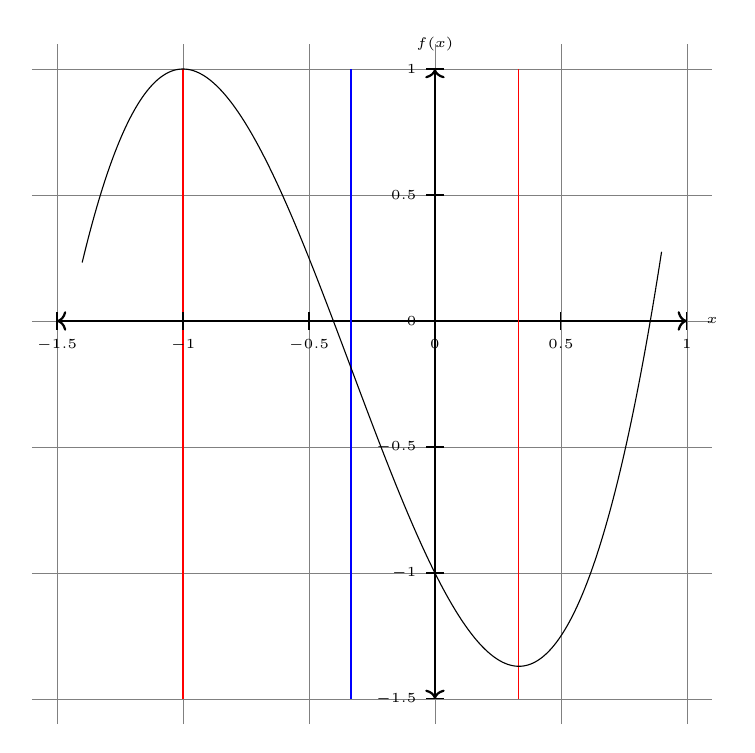
\begin{tikzpicture}[scale=3.2]
    			\draw[step=0.5cm,gray,very thin] (-1.6,-1.6) grid (1.1,1.1);
    			\draw[thick,->] (0,0) -- (1,0);
    			\draw[thick,->] (0,0) -- (0, 1);
    			\draw[thick,->] (0,0) -- (-1.5,0);
    			\draw[thick,->] (0,0) -- (0,-1.5);
    			\draw[thin,-,red] (-1,1) -- (-1,-1.5);
    			\draw[thin,-,red] (0.333,1) -- (0.333,-1.5);
    			\draw[thin,-,blue] (-0.333,1) -- (-0.333,-1.5);
    			\node[] at (1.1, 0) {\tiny $x$};
    			\node[] at (0, 1.1) {\tiny $f(x)$};
    			\foreach \x in {-1.5,-1,-0.5,0,0.5, 1}
       \draw (\x cm,1pt) -- (\x cm,-1pt) node[anchor=north] {\tiny $\x$};
    \foreach \y in {-1.5,-1,-0.5,0,0.5,1}
        \draw (1pt,\y cm) -- (-1pt,\y cm) node[anchor=east] {\tiny $\y$};
    
        \draw[variable=\t,domain=-1.4:0.9,samples=500] plot ({\t},{2*\t*\t*\t + 2*\t*\t - 2*\t - 1});
    
    		\end{tikzpicture}
	\end{figure}
    \end{soln}
    
    \newpage
    
    \item[11] Sketch a continuous function having all the following properties :
    \begin{description}
        \itemsep0.05em
        \item $f(-2)=8, f(0)=4, f(2)=0; f^{\prime}(-2) = f^{\prime}(2) = 0;$
        \item $f^{\prime}(x)>0$ for $\abs{x}>2$, $f^{\prime}(x)<0$ for $\abs{x} < 2$;
        \item $f^{\prime\prime}(x) < 0$ for $x<0$, $f^{\prime\prime}(x)>0$ for $x>0$.
    \end{description}
    
    \begin{soln}
        $f^{\prime} > 0$ in $(-\infty, -2) \cup (2, \infty)$ and thus $f$ is strictly increasing here. $f^{\prime} < 0$ in $(-2, 2)$ and thus $f$ is strictly decreasing here. Thus, $f$ has a local maximum at $-2$ and a local minimum at $-2$. The function values at these points are $8$ and $0$ respectively. Also, $f$ is convex in $(0, \infty)$ and concave in $(-\infty, 0)$ with an inflection point at $0$. Putting all these together, we can sketch a curve for $f$ as:
        
        \begin{figure}[!h]
		\centering
		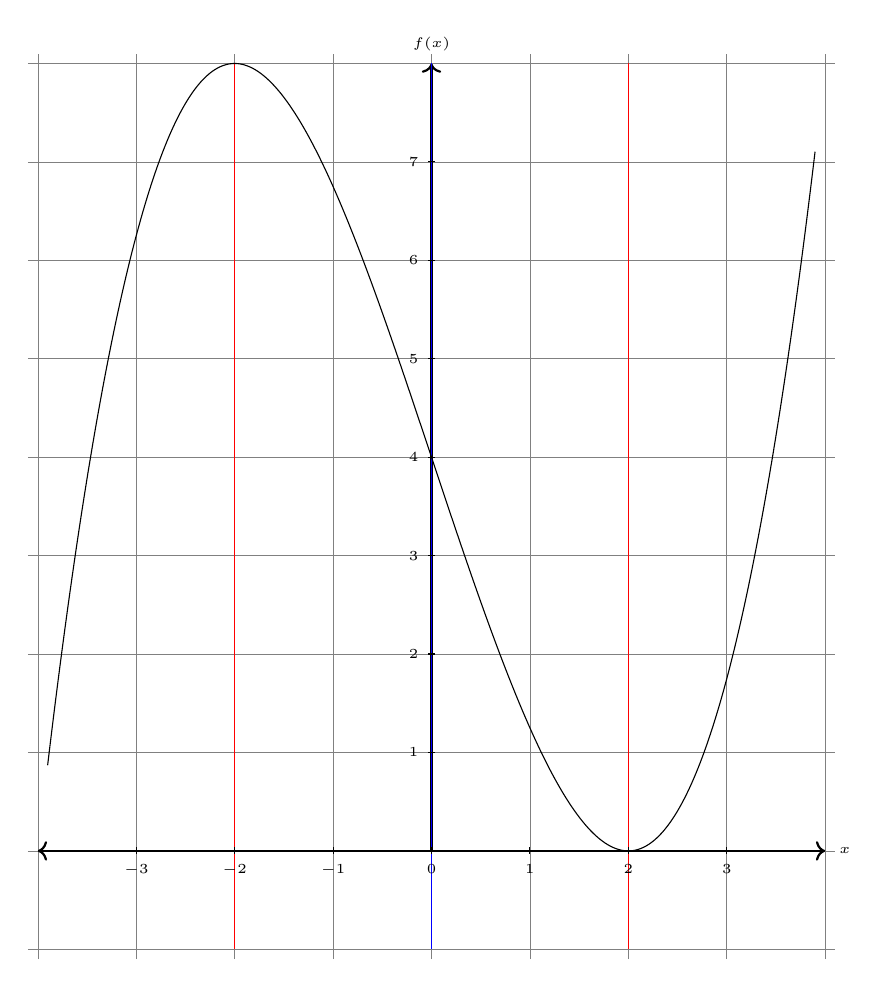
\begin{tikzpicture}[scale = 1.25]
			\draw[step=1cm,gray,very thin] (-4.1,-1.1) grid (4.1,8.1);
			\draw[thick,->] (0,0) -- (4,0);
			\draw[thick,->] (0,0) -- (0, 8);
			\draw[thick,->] (0,0) -- (-4,0);
			\draw[thin,-,red] (-2,-1) -- (-2,8);
			\draw[thin,-,red] (2,-1) -- (2,8);
			\draw[thin,-,blue] (0,-1) -- (0,8);
			\node[] at (4.2, 0) {\tiny $x$};
			\node[] at (0, 8.2) {\tiny $f(x)$};
			\foreach \x in {-3, ..., 3}
   \draw (\x cm,1pt) -- (\x cm,-1pt) node[anchor=north] {\tiny $\x$};
\foreach \y in {1, ...,7}
    \draw (1pt,\y cm) -- (-1pt,\y cm) node[anchor=east] {\tiny $\y$};

    \draw[variable=\t,domain=-3.9:3.9,samples=500] plot ({\t},{0.25*\t*\t*\t - 3*\t + 4});

		\end{tikzpicture}
	\end{figure}
    \end{soln}
    
    \newpage
    
    \textbf{Sheet 3.}
    
    \item[1 (ii)] Write down the Taylor expansion of $\arctan(x)$ around the point $0$. Also write a precise remainder term $R_n(x)$.
    
    \begin{soln}
        Let $f$ denote the arctangent function. Let $g$ denote its derivative
        \[
            g(x) = f^{\prime}(x) = \frac{1}{1+x^2}
        \]
        For $\abs{x} < 1$, we can expand the latter as a geometric series. Thus, we have
        \[
            g(x) = 1 - x^2 + x^4 - x^6 + \ldots = \sum_{k=0}^{\infty} (-1)^k x^{2k}
        \]
        for $\abs{x} < 1$. Let us now evaluate the $n^{\text{th}}$ derivative of $f$ at $x=0$. For $n \geq 1$, we have
        \[
            f^{(n)} = g^{(n-1)}
        \]
        where $f^{(r)}$ and $g^{(r)}$ denote the $r^{\text{th}}$ derivatives of $f$ and $g$ respectively. To evaluate the derivatives of $g$, we will consider two cases. First, we will evaluate all odd derivatives (derivatives of the order $2n-1$). On differentiating $g$, $r$ times, we will be left with a power series where the powers of $x$ are of the form $(2k-r)$ \textcolor{blue}{for integer $k$}. When $r$ is odd, no exponent of $x$ vanishes. As a result, all the terms of the power series vanish when we plug in $x=0$. Thus, all odd derivatives of $g$ vanish at $0$. I leave it to you to compute the even order derivatives at $x=0$. The derivatives of $g$ at $0$ are then given by
        \[
            g^{(2n-1)}(0) = 0, \quad g^{(2n)}(0) = (-1)^n \cdot (2n)!
        \]
        for $n \geq 1$. Now, we have
        \[
            f^{2n}(0) = g^{(2n-1)}(0) = 0
        \]
        and
        \[
            f^{(2n-1)}(0) = g^{(2n-2)}(0) = (-1)^{n-1} \cdot (2n-2)!
        \]
        for $n \geq 1$. \textcolor{blue}{We shall first compute the zeroth Taylor Polynomial. We have}
        \[
            \textcolor{blue}{T_0(x) = f(0) = 0}
        \]  
        Let us now compute the $n^{\text{th}}$ Taylor polynomial $T_n(x)$ of $f$ at $0$ \textcolor{blue}{for $n \geq 1$}. Define $M \vcentcolon= \left\lfloor \left( \frac{n+1}{2} \right)  \right\rfloor$.   \textcolor{blue}{ For $n \geq 1$}, we then have
        \[
            T_n(x) = \sum_{k=0}^{n} \frac{f^{(k)}(0)}{k!} x^k
        \]
        where $f^{(0)} = f$. With a bit of manipulation, we can write 
        \[
            T_n(x) = \sum_{k=1}^{M} \frac{(-1)^{k-1} \cdot (2k-2)!}{(2k-1)!} \cdot x^{2k-1}
        \]  
        Thus, the $n^{\text{th}}$ Taylor polynomial for $\arctan$ at $0$ is given by
        \[
            T_n(x) = \sum_{k=1}^{M} \frac{(-1)^k}{2k-1} x^{2k-1} \quad , \quad M = \left\lfloor \left( \frac{n+1}{2} \right) \right\rfloor
        \]
        
        Writing it out in a neater way, we have
        \[
            T_{2n-1}(x) = x - \frac{x^3}{3} + \ldots + \frac{(-1)^{n-1}}{2n-1} x^{2n-1} 
        \]
        and 
        \[
            T_{2n}(x) = T_{2n-1}(x)
        \]
        
        The remainder term is then just the difference of the arctangent function at $x$ and its Taylor polynomial. More precisely, we have
        \[
            R_n(x) = \arctan(x) - \sum_{k=0}^{M} \frac{(-1)^k}{2k-1} x^{2k-1}
        \]
        with $M$ defined as previously. Let us now calculate the remainder term $R_{2n-1}(x)$ more explicitly. We have
        \[
            \arctan^{\prime} = \textcolor{cyan}{1 - x^2 + x^4 + \ldots + (-1)^{n-1} x^{2n-2}} + (-1)^n x^{2n} \left[1 - x^2 + x^4 - \ldots \right]
        \]
        \[
            \therefore \arctan^{\prime} = \textcolor{cyan}{1 - x^2 + x^4 + (-1)^{n-1} x^{2n-2}} + (-1)^{n} \frac{x^{2n}}{1+x^2}
        \]
        On integrating both sides from $0$ to $x$, the cyan-coloured term just becomes $T_{2n-1}(x)$. (Verify!) Thus, we have
        \[
            \arctan(x) = T_{2n-1}(x) + (-1)^n \int_{0}^{x} \frac{t^{2n}}{1+t^2} \, \D t
        \]
        Thus, 
        \[
            R_{2n-1}(x) = (-1)^n \int_{0}^{x} \frac{t^{2n}}{1+t^2} \, \D t
        \]
        and 
        \[
            R_{2n}(x) = R_{2n-1}(x)
        \]
    \end{soln}
    
    \newpage
    
    \item[2] Write down the Taylor series of the polynomial $x^3 - 3x^2 + 3x - 1$ about the point $1$.
    \begin{soln}
        The Taylor series is just $(x-1)^3$. Let us see why. We wish to expand 
        \[
            f(x) = x^3 - 3x^2 + 3x -1
        \]
        about the point $a=1$. We have
        \[
            f(1) = 0
        \]
        \[
            f^{(1)}(1) = 0
        \]
        \[
            f^{(2)}(1) = 0
        \]
        \[
            f^{(3)}(1) = 6
        \]
        \[
            f^{(n)}(1) = 0 \; \text{ for all } n \geq 4
        \]
        Thus, we have
        \[
            P_0(x) = P_1(x) = P_2(x) = 0
        \]
        \[
            P_3(x) = \frac{6}{3!} (x-1)^3 = (x-1)^3
        \]
        and
        \[
            P_n(x) = P_3(x) \; \text{ for all } n \geq 4
        \]
        We also have
        \[
            R_n(x) \vcentcolon= f(x) - P_n(x) = 0 \; \text{ for all } n \geq 3
        \]
        Thus, $R_n(x) \to 0$ for \textbf{all} $x$. Thus, the Taylor series of the function about the point $1$ is simply given by $(x-1)^3$.
    \end{soln}
    
    \item[4] Consider the series $\sum\limits_{k=0}^{\infty} \ddfrac{x^k}{k!}$ for a fixed $x$. Prove that it converges as follows. Choose $N > 2\textcolor{blue}{\abs{x}}$. We see that for $n > N$, 
    \[
        \textcolor{blue}{\abs{\frac{x^{n+1}}{(n+1)!}} < \frac{1}{2} \cdot \abs{\frac{x^n}{n!}}}
    \]
    It should now be relatively easy to show that the given series is Cauchy, and hence (by the completeness of $\mathbb{R}$) is convergent.
    
    \begin{soln}
        Let the partial sums of the series be denoted as $S_m(x)$. That is,
        \[
            S_m(x) \vcentcolon= \sum_{k=0}^{m} \frac{x^k}{k!}
        \]
        We wish to show that the difference $\abs{S_m(x) - S_n(x)}$ can be made arbitrarily small whenever $m$ and $n$ are sufficiently large. Assume that $m>n>N$. We see that
        \[
            \abs{S_m(x) - S_n(x)} = \abs{\sum_{k=n+1}^{m}\frac{x^k}{k!}} \leq \abs{\frac{x^n}{n!}} \left( \frac{1}{2} + \frac{1}{4} + \ldots + \frac{1}{2^{m-n}} \right) \leq \abs{\frac{x^n}{n!}} \textcolor{blue}{< \abs{\frac{x^N}{N!}}}
        \]
        Now for any $\epsilon>0$, we can pick $\textcolor{blue}{N}$ large enough such that
        \[
            \abs{\frac{x^N}{N!}} < \epsilon
        \]
        This is possible because the sequence
        \[
            a_n = \frac{\abs{x}^n}{n!} 
        \]
        is convergent (it is eventually decreasing and bounded below) and its limit is $0$. Thus, for all $m>n>N$, we have
        \[
            \abs{S_m(x) - S_n(x)} < \epsilon
        \]
        Hence, the given series is Cauchy and thus convergent.
        
        (\underline{Remark}: During the tutorial session, I had showed that the term $\abs{S_m(x) - S_n(x)}$ can be made arbitrarily small by picking $\textcolor{blue}{n}$ large enough. However, this is incorrect! We want to show that the term is smaller than $\epsilon$ for any $n,m$ greater than $N$. So really we have to make $\textcolor{blue}{N}$ large enough and conclude. This is what I have now done.)
    \end{soln}
    
    \newpage
    
    \item[5] Using Taylor series, write down a series for the integral
    \[
        \int \frac{e^x}{x} \, \D x
    \]
    
    \begin{soln}
        We will assume that a Taylor series can be integrated term by term and then proceed. Recall that the Taylor series for $e^x$ is given by
        \[
            e^x = \sum_{k=0}^{\infty} \frac{x^k}{k!}
        \]
        We have
        \begin{align*}
            \int \frac{e^x}{x} \, \D x &= \int \left( \frac{1}{x} + \sum_{k=1}^{\infty} \frac{x^{k-1}}{k!} \right) \, \D x \\
            &= \int \frac{1}{x} \, \D x + \int \left( \sum_{k=1}^{\infty} \frac{x^{k-1}}{k!} \right) \, \D x
        \end{align*}
        Since the latter term is a Taylor series, we can integrate it term by term to obtain
        \[
             \int \frac{e^x}{x} \, \D x = \log x + \sum_{k=1}^{\infty} \left( \int \frac{x^{k-1}}{k!} \, \D x \right)
        \]
        Thus, a series representation of the integral is given by
        \[
            \int \frac{e^x}{x} \, \D x = \log x + \sum_{k=1}^{\infty} \frac{x^k}{k \cdot k!}
        \]
    \end{soln}
\end{enumerate}

\newpage\section{Week 4}
\begin{center}
	16th December, 2020
\end{center}
\textbf{Sheet 4.}

\begin{enumerate}[leftmargin=*]
    \itemsep0.5em
    \item[2 (a)] Let $f \colon [a,b] \to \mathbb{R}$ be Riemann integrable and $f(x) \geq 0$ for all $x \in [a,b]$. Show that $\displaystyle\int_a^b f(x) \, \D x \geq 0$. Further, if $f$ is continuous and $\displaystyle\int_a^b f(x) \, \D x = 0$, show that $f(x) = 0$ for all $x \in [a,b]$.
    
    \begin{soln}
        Let $P = \left\{ a=x_0 <  x_1 < \ldots < x_n = b \right\}$ denote a partition of $[a,b]$. Define $\Delta x_i = x_i - x_{i-1}$ for $1 \leq i \leq n$. Further, we define
        \[
            m_i = \inf \left\{ f(x) \colon x_{i-1} \leq x \leq x_i \right\}
        \]
        Since $f(x) \geq 0$ for all $x \in [a,b]$, it follows that $m_i \geq 0$ for all $i$. The lower sum is now defined as
        \[
            L(P,f) = \sum_{i=1}^{n} m_i \Delta x_i
        \]
        Since $m_i \geq 0$ and $\Delta x_i > 0$ for all $i$, it follows that $L(P, f) \geq 0$ for any partition $P$. Thus, we also see that $L(f) \geq 0$ since $L(f)$ is the supremum of $L(P,f)$ over all partitions $P$. Since $f$ is Riemann integrable, we have
        \[
            \int_a^b f(x) \, \D x = L(f) \geq 0
        \]
        as desired. 
        
        \medskip
        
        Now, let us further assume that $f$ is continuous and that $\int_a^b f(x) \, \D x = 0$. If $f$ is not identically zero, then there exists $c \in [a,b]$ such that $f(c) > 0$. Continuity of $f$ implies that there exists a $\delta > 0$ such that, if $x \in [a,b]$, 
        \[
            \abs{x-c} < \delta \implies \abs{f(x) - f(c)} < \frac{f(c)}{2} \implies f(x) > \frac{f(c)}{2}
        \]
        We may now assume $c \in {\color{red}(}a,b{\color{red})}$ without any loss of generality \footnote{If $c=a$ or $c=b$, then we can pick another point $\Tilde{c}$ in $(a,b)$ such that $f(\Tilde{c}) \neq 0$.} Further, pick $\delta > 0$ small enough so that $(c-\delta, c+\delta) \subset (a,b)$. Now, consider the partition
        \[
            P = \left\{ a, c-\frac{\delta}{2}, c+\frac{\delta}{2}, b \right\}
        \]
        Since we have
        \[
            \inf\limits_{x \in [c-\frac{\delta}{2}, c+\frac{\delta}{2}]} f(x) \geq \frac{f(c)}{2}
        \]
        it follows that
        \[
            L(f) \geq L(P,f) \geq \frac{f(c) \delta}{2} > 0
        \]
        Further, if $f$ is Riemann integrable, we have that its integral over $[a,b]$ is equal to $L(f)$, which is strictly positive - a contradiction! Hence, $f$ must be identically zero.
    \end{soln}
    
            
        \medskip
        \hrule
        
        \medskip
        
    
    \textcolor{blue}{\underline{Alternate.} (easier)} 
    
    \begin{soln}
        Consider the trivial partition $P_0 = {a,b}$ of $[a,b]$. Since $f(x) \geq 0$ for all $x \in [a,b]$, we have
        \[
            \inf_{x \in [a,b]} f(x) \geq 0
        \]
        We have
        \[
            L(f, P_0) = \left[ \inf_{x \in [a,b]} f(x) \right] \cdot (b-a) \geq 0
        \]
        and 
        \[
            L(f) \geq L(f, P_0) \geq 0
        \]
        Since $f$ is Riemann integrable, its integral is $L(f)$, which is non-negative, as desired.
        
        \medskip

        For the second part, define $F \colon [a,b] \to \mathbb{R}$ as
        \[
            F(x) = \int_a^x f(t) \, \D t
        \]
        Since $f$ is continuous, we get that $F$ is differentiable with $F^{\prime} = f$, from the Fundamental Theorem of Calculus (Part 1).
        Since $f \geq 0$, we have $F^{\prime} \geq 0$ and hence, $F$ is increasing. This implies that for all $x \in [a,b]$, we have
        \[
            F(a) \leq F(x) \leq F(b)
        \]
        However, since $F(a) = 0 = F(b)$, we get that $F$ is constant and hence, 
        \[
            f(x) = F^{\prime}(x) = 0
        \]
        for all $x \in [a,b]$, as desired.
    \end{soln}
    
    \newpage
    
    \item[2 (b)] Give an example of a Riemann integrable function on $[a,b]$ such that $f(x) \geq 0$ for all $x \in [a,b]$ and $\int_a^b f(x) \, \D x = 0$, but $f(x) \neq 0$ for some $x \in [a,b]$.
    
    \begin{soln}
        As we saw in the previous question, no continuous function can satisfy these conditions. Thus, we must look for a discontinuous function. We define $f$ on $[0,1]$ as follows:
        \[
            f(x) = \begin{cases}
                0 & \text{when $x \neq \frac{1}{2}$} \\
                1 & \text{when $x = \frac{1}{2}$}
            \end{cases}
        \]
        Since $f$ has only finitely many discontinuities, it is Riemann integrable. Also, $f(x) \geq 0$ for all $x \in [0,1]$. Further, it is easy to show that its Riemann integral over the interval is $0$. Lastly, we have $f(\frac{1}{2}) = 1 \neq 0$. Thus, $f(x) \neq 0$ for some $x \in [0,1]$. Hence, this $f$ satisfies our desired conditions.
    \end{soln}
    
    \newpage


    \item[3] Evaluate $\lim\limits_{n \to \infty} S_n$ by showing that $S_n$ is an \textcolor{red}{\sout{approximate}} appropriate Riemann sum of a suitable function over a suitable interval.
    
        \begin{multicols}{2}
    \begin{enumerate}[leftmargin=*]
        \item[(ii)] $S_n = \sum\limits_{i=1}^{n} \ddfrac{n}{i^2 + n^2}$
        \item[(iv)] $S_n = \dfrac{1}{n} \sum\limits_{i=1}^n \cos \dfrac{i\pi}{n}$
    \end{enumerate}
    \end{multicols}
    
    We shall use the following theorem for both the parts. 
    
    \begin{thm*}
        Let $f \colon [a,b] \to \mathbb{R}$ be Riemann integrable. Suppose that $(P_n, T_n)$ be a sequence of tagged partitions of $[a,b]$ such that $\norm{P_n} \to 0$. Then, 
        \[
            R(P_n, T_n, f) \to \int_a^b f(t) \, \D t
        \]
    \end{thm*}
    
    \begin{enumerate}[leftmargin=*]
    \item[(ii)]
    \begin{soln}
        Consider $f \colon [0,1] \to \mathbb{R}$ defined as $f(x) \vcentcolon= \arctan(x)$. Then, we have
        \[
            f^{\prime}(x) = \frac{1}{1+x^2}
        \]
        Since $f^{\prime}$ is continuous on $[0,1]$, it is Riemann integrable on $[0,1]$. Let $P_n \vcentcolon= \left\{ x_i = \frac{i}{n} \colon 0 \leq i \leq n \right\}$ be a tagged partition of $[0,1]$ for $n \in \mathbb{N}$ and let $T_n \vcentcolon= \left\{ t_i = \frac{i}{n} \colon 1 \leq i \leq n\right\}$ denote the tags of the partition. 
        
        \medskip
        
        We have $\Delta x_i = x_{i} - x_{i-1} = \frac{1}{n}$ for all $1 \leq i \leq n$. The Riemann sum corresponding to this tagged partition is given by 
        \begin{align*}
            R(P_n, T_n, f^{\prime}) = \sum_{i=1}^{n} f^{\prime}(t_i) \Delta x_i &= \sum_{i=1}^n \frac{1}{1+t_i^2} \cdot \frac{1}{n} \\
            &= \sum_{i=1}^n \frac{1}{1 + \left(\frac{i}{n} \right)^2 } \cdot \frac{1}{n} \\
            &= \sum_{i=1}^n \frac{n}{i^2 + n^2} = S_n
        \end{align*}
        
        Thus, $R(P_n, T_n, f^{\prime}) = S_n$ for all $n \geq 1$. Moreover, 
        \[
            \norm{P_n} = \max \left\{ x_i - x_{i-1} \colon 1 \leq i \leq n \right\} = \frac{1}{n}
        \]
        Clearly, we have
        \[
            \lim_{n \to \infty} \norm{P_n} = 0
        \]
        and thus,
        \[
            \lim_{n \to \infty} S_n = \int_0^1 f^{\prime}(x) \, \D x
        \]
        From the Fundamental Theorem of Calculus (Part $2$), we have that
        \[
            \lim_{n \to \infty} S_n = \int_0^1 f^{\prime}(x) \, \D x = f(1) - f(0) = \boxed{\frac{\pi}{4}}
        \]
        \end{soln}
        
        \item[(iv)] 
        \begin{soln}
    
        Consider $f : [0,1] \to \mathbb{R}$ defined as 
        \[
            f(x) \vcentcolon= \frac{1}{\pi} \sin(\pi x) 
        \]
        We then have $f^{\prime}(x) = \cos(\pi x)$. Since $f^{\prime}$ is continuous on $[0,1]$, it is Riemann integrable on $[0,1]$. Let $P_n \vcentcolon= \left\{ x_i = \frac{i}{n} \colon 0 \leq i \leq n \right\}$ be a tagged partition of $[0,1]$ for $n \in \mathbb{N}$ and let $T_n \vcentcolon= \left\{ t_i = \frac{i}{n} \colon 1 \leq i \leq n\right\}$ denote the tags of the partition. 
        
        \medskip
        
        We have $\Delta x_i = x_{i} - x_{i-1} = \frac{1}{n}$ for all $1 \leq i \leq n$. The Riemann sum corresponding to this tagged partition is given by 
        \begin{align*}
            R(P_n, T_n, f^{\prime}) = \sum_{i=1}^{n} f^{\prime}(t_i) \Delta x_i &= \sum_{i=1}^n \cos(\pi t_i) \cdot \frac{1}{n} \\
            &= \frac{1}{n} \sum\limits_{i=1}^n \cos \frac{i\pi}{n} = S_n
        \end{align*}
        
        Thus, $R(P_n, T_n, f^{\prime}) = S_n$ for all $n \geq 1$. Moreover, 
        \[
            \norm{P_n} = \max \left\{ x_i - x_{i-1} \colon 1 \leq i \leq n \right\} = \frac{1}{n}
        \]
        Clearly, we have
        \[
            \lim_{n \to \infty} \norm{P_n} = 0
        \]
        and thus,
        \[
            \lim_{n \to \infty} S_n = \int_0^1 f^{\prime}(x) \, \D x
        \]
        From the Fundamental Theorem of Calculus (Part $2$), we have that
        \[
            \lim_{n \to \infty} S_n = \int_0^1 f^{\prime}(x) \, \D x = f(1) - f(0) = \boxed{0}
        \]
        \end{soln}
    \end{enumerate}
    
    \newpage
    
    \item[4(b)] Compute $\dfrac{\D F}{\D x}$ if for $x \in \mathbb{R}$, 
    \begin{multicols}{2}
    \begin{enumerate}[leftmargin=*]
        \item[(i)] $F(x) = \displaystyle\int_1^{2x} \cos\left( t^2 \right) \, \D t$
        \item[(ii)] $F(x) = \displaystyle\int_0^{x^2} \cos(t) \, \D t$
    \end{enumerate}
    \end{multicols}
    
    \begin{soln}
        Before solving these two subparts, I will first prove a short lemma. 
        \begin{lem*}
            Let $f \colon \mathbb{R} \to \mathbb{R}$ be continuous and let $v \colon \mathbb{R} \to \mathbb{R}$ be differentiable. Let $F \colon \mathbb{R} \to \mathbb{R}$ be defined as
            \[
                F(x) \vcentcolon= \int_{0}^{v(x)} f(t) \, \D t
            \]
            Then, 
            \[
                F^{\prime}(x) = f\left( v(x) \right) \cdot v^{\prime}(x)
            \]
        \end{lem*}
        
        \begin{proof}
            First, we define $G \colon \mathbb{R} \to \mathbb{R}$ as 
            \[
                G(x) \vcentcolon= \int_0^x f(t) \, \D t
            \]
            Then, $G^{\prime} = f$ by the Fundamental Theorem of Calculus (Part $1$). Now,
            \[
                F(x) = G\left( v(x) \right)
            \]
            A simple application of chain rule yields
            \[
                F^{\prime}(x) = f\left( v(x) \right) \cdot v^{\prime}(x)
            \]
            as desired.
        \end{proof}
        
        \begin{enumerate}[leftmargin=*]
            \item[(i)] We have $v(x) = 2x$ and $f(t) = \cos(t^2)$. It thus follows from the above lemma that
            \[
                \frac{\D F}{\D x} = \cos \left( (2x)^2 \right) \cdot \left( 2x \right)^{\prime} = \boxed{2\cos\left( 4x^2 \right)}
            \]
            \item[(ii)] We have $v(x) = x^2$ and $f(t) = \cos(t)$. It thus follows from the above lemma that
            \[
                \frac{\D F}{\D x} = \cos \left( x^2 \right) \cdot \left( x^2 \right)^{\prime}= \boxed{2x \cos\left( x^2 \right)}
            \]
        \end{enumerate}
    \end{soln}
    
    \newpage
    
    \item[6] Let $f \colon \mathbb{R} \to \mathbb{R}$ be continuous and $\lambda \in \mathbb{R}, \lambda \neq 0$. For $x \in \mathbb{R}$, let
    \[
        g(x) = \frac{1}{\lambda} \int_0^x f(t) \sin{\lambda(x-t)} \, \D t
    \]
    Show that $g^{\prime\prime}(x) + \lambda^2 g(x) = f(x)$ for all $x \in \mathbb{R}$ and $g(0) = g^{\prime}(0) = 0$.
    
    \begin{soln}
        We will first make use of the identity $\sin{(A-B)} = \sin{A}\cos{B} - \cos{A}\sin{B}$. We have
        \begin{align*}
            g(x) &= \frac{1}{\lambda} \int_0^x f(t) \sin{\lambda(x-t)} \, \D t \\
            &= \frac{1}{\lambda} \int_0^x f(t) \left( \sin{\lambda x} \cos{\lambda t} - \cos{\lambda x} \sin{\lambda t} \right) \, \D t \\
            &= \frac{1}{\lambda} \sin{\lambda x} \int_0^x f(t) \cos{\lambda t} \, \D t - \frac{1}{\lambda} \cos{\lambda t} \int_0^x f(t) \sin{\lambda t} \, \D t
        \end{align*}
        
        On applying the product rule and Fundamental Theorem of Calculus (Part $1$), we get
        \begin{align*}
            g^{\prime}(x) &= \cos{\lambda x} \int_0^x f(t) \cos{\lambda t} \, \D t + \cancel{\frac{1}{\lambda} \sin{\lambda x} \cdot f(x) \cdot \cos{\lambda x}} \\
            &+ \sin{\lambda x} \int_0^x f(t) \sin{\lambda t} \, \D t - \cancel{ \frac{1}{\lambda} \sin{\lambda x} \cdot f(x) \cdot \cos{\lambda x}}
        \end{align*}
        \[
            \therefore \; g^{\prime}(x) = \cos{\lambda x} \int_0^x f(t) \cos{\lambda t} \, \D t + \sin{\lambda x} \int_0^x f(t) \sin{\lambda t} \, \D t
        \]
        It is now easy to verify that both $g(0)$ and $g^{\prime}(0)$ are indeed $0$. We will differentiate $g^{\prime}$ in a similar manner to obtain
        \begin{align*}
            g^{\prime \prime}(x) &= -\lambda \sin{\lambda x} \int_0^x f(t) \cos{\lambda t} \, \D t + f(x) \cos^2{\lambda x} \\
            &+ \lambda \cos{\lambda x} \int_0^x f(t) \sin{\lambda t} \, \D t + f(x) \sin^2{\lambda x} \\
            &= f(x) - \lambda^2 \left( \frac{1}{\lambda} \int_0^x f(t) \left( \sin{\lambda x} \cos{\lambda t} - \cos{\lambda x} \sin{\lambda t} \right) \, \D t\right) \\
            &= f(x) - \lambda^2 g(x)
        \end{align*}
        It thus follows that $g^{\prime\prime}(x) + \lambda^2 g(x) = f(x)$ for all $x \in \mathbb{R}$, as desired.
    \end{soln}
\end{enumerate}

\newpage
\section{Week 5}
\begin{center}
    23rd December, 2020
\end{center}

\textbf{Sheet 5}

\begin{enumerate}[leftmargin=*]
    \itemsep0.5em
    \item[2] Describe the level curves and contour lines for the following functions corresponding to the values $c=-3,-2,-1,0,1,2,3,4$.
    \begin{multicols}{2}
        \begin{enumerate}[leftmargin=*]
            \item[(ii)] $f(x,y) = x^2 + y^2$
            \item[(iii)] $f(x,y) = xy$
        \end{enumerate}
    \end{multicols}
    
    \begin{enumerate}[leftmargin=*]
        \item[(ii)] \begin{soln} \textcolor{blue}{($x^2 + y^2 = c$)}
        
            For $c=-3,-2,-1$, level curves and contour lines are empty sets. For $c=0$, the level curve is the point $(0,0) \in \mathbb{R}^2$ and the contour line is the point $(0,0,0) \in \mathbb{R}^3$. For any $c \in \{1,2,3,4\}$, the level curve is a circle in the $xy$ plane, centered at the origin, with radius $\sqrt{c}$. More precisely, the level curve is the set $L = \left\{ (x,y) \in \mathbb{R}^2 \mid x^2 + y^2 = c \right\}$. The contour line is a cross-section in $\mathbb{R}^3$ of the paraboloid $z = x^2 + y^2$ by the plane $z=c$. That is, a circle in the plane $z=c$, centered at $(0,0,c)$ and with radius $\sqrt{c}$. More precisely, the contour line is the set $L \times \{c\}$.
        \end{soln}
        
        \item[(iii)] \begin{soln}\textcolor{blue}{($xy=c$)}
        
            %For $c=-3,-2,-1$, the level curves are rectangular hyperbolas $xy=c$ with branches in the second and fourth quadrant. For $c=1,2,3,4$, the level curves are rectangular hyperbolas $xy=c$ with branches in the first and third quadrant. For $c=0$, the level curve is the union of the $x$ and $y$ axes in the $xy$-plane, while the contour line is the union of the $x$ and $y$ axes in the $xyz$-space. For non-zero $c$, the contour lines are cross-sections of the hyperboloid $z=xy$ by the plane $z=c$. That is, these are rectangular hyperbolas in the plane $z=c$.
            
            For $c = 0$, the level set is the union of the $x$ and $y$ axes in the $xy$-plane. Precisely, this is the set $L = \left\{ (x,y) \in \mathbb{R}^2 \mid  x = 0 \text{ or } y =0\right\}$. The contour line corresponding to $c=0$ is the union of the $x$ and $y$ axes in the $xyz$-space. This is the set $L \times \{0\}$. For any non-zero $c$, the level curve is the rectangular hyperbola $xy = c$ and the contour line is the cross-section of the hyperboloid $z = xy$ by the plane $z=c$. More precisely, the level curve is the set $L = \left\{ (x,y) \in \mathbb{R}^2 \mid xy = c \right\}$ and the contour line is the set $L \times \{c\}$. For negative $c$, the level curve (and the contour line) has branches in the second and fourth quadrant while for positive $c$, the level curve (and the contour line) has branches in the first and third quadrants.
        \end{soln}
    \end{enumerate}
    
    \newpage
    
    \item[4] Suppose $f,g \colon \mathbb{R} \to \mathbb{R}$ are continuous functions. Show that each of the following functions of $(x,y) \in \mathbb{R}^2$ are continuous. 
    
    \begin{multicols}{2}
        \begin{enumerate}[leftmargin=*]
            \item[(i)] $f(x) \pm g(y)$
            \item[(ii)] $f(x) g(y)$
        \end{enumerate}
    \end{multicols}
    \begin{multicols}{2}
        \begin{enumerate}[leftmargin=*]
            \item[(iii)] $\max\left\{ f(x), g(y) \right\}$
            \item[(iv)] $\min\left\{ f(x), g(y) \right\}$
        \end{enumerate}
    \end{multicols}
    
    \begin{soln}
        We will use sequential criterion of continuity. Just to recall:
        
        \begin{thm*}[Sequential Criterion]
            Let $f \colon \mathbb{R}^2 \to \mathbb{R}$ be a function. Then, $f$ is continuous at $(x_0, y_0)$ if and only if for every sequence $\left( (x_n, y_n) \right)$ converging to $(x_0, y_0)$, we have 
            \[
                \lim_{n \to \infty} f\left( x_n, y_n \right) = f(x_0, y_0)
            \]
        \end{thm*}
        
        Let $(x_0, y_0)$ be an arbitrary point of $\mathbb{R}^2$. Let $(x_n, y_n)$ be an arbitrary sequence in $\mathbb{R}^2$ such that $(x_n, y_n) \to (x_0, y_0)$. We then have $x_n \to x_0$ and $y_n \to y_0$. Since $f$ and $g$ are continuous, it follows that $f(x_n) \to f(x_0)$ and $g(y_n) \to g(y_0)$. For (i) and (ii), note that we can now use algebra of limits to conclude that the given functions are indeed continuous. 
        
        \medskip
        
        For (iii) and (iv), note the following:
        \[
            \max\left\{ f(x), g(y) \right\} = \frac{f(x) + g(y)}{2} + \frac{\abs{f(x) - g(y)}}{2}
        \]
        \[
            \min\left\{ f(x), g(y) \right\} = \frac{f(x) + g(y)}{2} - \frac{\abs{f(x) - g(y)}}{2}
        \]
        Again, consider $\left( (x_n, y_n) \right)$ to be an arbitrary sequence converging to $(x_0, y_0)$. We then have $x_n \to x_0$ and $y_n \to y_0$. From the continuity of $f,g$ it follows that $f(x_n) \to f(x_0)$ and $g(y_n) \to g(y)$. Thus, we have
        \[
            f(x_n) + g(y_n) \to f(x_0) + g(y_0)
        \]
        Since the modulus function is continuous, we also have
        \[
            \abs{f(x_n) + g(y_n)} \to \abs{f(x_0) + g(y_0)}
        \]
        It then follows that
        \[
            \frac{f(x_n) + g(y_n)}{2} + \frac{\abs{f(x_n) - g(y_n)}}{2} \longrightarrow \frac{f(x_0) + g(y_0)}{2} + \frac{\abs{f(x_0) - g(y_0)}}{2}
        \]
        which can be rewritten as
        \[
            \max\left\{ f(x_n), g(y_n) \right\} \to \max\left\{ f(x_0), g(y_0) \right\}
        \]
        concluding the proof for (iii). Similarly, the proof for (iv) follows.
        
        \medskip
        
        Since the point $(x_0, y_0)$ was arbitrary, it follows that the given functions are continuous on all of $\mathbb{R}^2$.
    \end{soln}
    
    \newpage
    
    \item[6 (ii)] Examine the following functions for the existence of partial derivatives at $(0,0)$. The expressions below give the value for $(x,y) \neq (0,0)$. At $(0,0)$, the value should be taken to be zero.
    \[
        \frac{\sin^2\left( x+y \right)}{\abs{x} + \abs{y}}
    \]
    
    \begin{soln}
        Let $f \colon \mathbb{R}^2 \to \mathbb{R}$ be the function given. That is, 
        \[
            f(x,y) = \begin{cases}
                \dfrac{\sin^2\left( x+y \right)}{\abs{x} + \abs{y}} & (x,y) \neq (0,0) \\
                0 & (x,y) = (0,0)
            \end{cases}
        \]
        
        For $h \neq 0$, we have
        \[
            \frac{f(h,0) - f(0,0)}{h}
            = \left( \frac{\sin^2{h}}{h\abs{h}} \right)
        \]
        
        It is easy to show that the above limit (as $h$ goes to $0$) does not exist (Take strictly positive and strictly negative sequences converging to zero). Hence, we see that $\dfrac{\partial f}{\partial x_1}(0,0)$ does not exist. Similar arguments show that the second partial does not exist either.
    \end{soln}
    
    \newpage
    
    \item[8] Let $f$ be defined as 
    \[
        f(x,y) = \begin{cases}
            x \sin{\left( 1/x \right)} + y \sin{\left( 1/y \right)} & x \neq 0, y \neq 0 \\
            x \sin{\left( 1/x \right)} & x \neq 0, y = 0 \\
            y \sin{\left( 1/y \right)} & x=0, y \neq 0 \\
            0 & x=0, y=0
        \end{cases}
    \]
    Show that none of the partial derivatives of $f$ exist at $(0,0)$ although $f$ is continuous at $(0,0)$.
    
    \begin{soln}
        Let us first show that the given function is continuous at $(0,0)$. Let $(x_n,y_n)$ be a sequence in $\mathbb{R}^2$ such that $(x_n, y_n) \to (0,0)$. This gives us that $x_n \to 0$ and $y_n \to 0$. Now, note that
        \[
            0 \leq \abs{f(x_n, y_n)} \leq \abs{x_n} + \abs{y_n}
        \]
        for all $(x_n, y_n) \in \mathbb{R}^2$. Since $(x_n, y_n) \to (0,0)$, we get that $f(x_n, y_n) \to 0 = f(0,0)$. Thus, the function is continuous at $(0,0)$.
        
        \medskip
        
        Let us now show that neither partial derivatives of $f$ at $(0,0)$ exist. For $h \neq 0$, we have
        \[
            \frac{f(h,0) - f(0,0)}{h} = \sin{\frac{1}{h}}
        \]
        The limit of the above expression as $h \to 0$, does not exist. Similar arguments show that the second partial derivative does not exist either.
    \end{soln}
    
    \newpage
    
    \item[10] Let $f \colon \mathbb{R}^2 \to \mathbb{R}^2$ be defined as 
    \[
        f(x,y) = \begin{cases}
            \frac{y}{\abs{y}} \sqrt{x^2 + y^2} & y \neq 0 \\
            0 & y = 0
        \end{cases}
    \]
    
    Show that $f$ is continuous at $(0,0)$, $\nabla_{\underline{u}} f(0,0)$ exists for every \textcolor{blue}{unit} vector $\textbf{u}$ and yet, $f$ is not differentiable at $(0,0)$. 
    
    \begin{soln}
        First, we will show that $f$ is indeed continuous at $(0,0)$. We will now use the $\epsilon$-$\delta$ condition (it's easier to work with in this case). Note that we have
        \[
            \abs{f(x,y) - f(0,0)} = \begin{cases}
                \sqrt{x^2+y^2} & y \neq 0 \\
                0 & y = 0
            \end{cases}
        \]
        Thus, in general, we have
        \[
            \abs{f(x,y) - f(0,0)} \leq \sqrt{x^2 + y^2}
        \]
        Now, given any $\epsilon > 0$, setting $\delta \vcentcolon= \epsilon$ works.
        
        \medskip
        
        Let $\underline{u} = (u_1, u_2)$ be a unit vector in $\mathbb{R}^2$. If $u_2 \neq 0$, then for $t\neq 0$, we have
        \begin{align*}
            \frac{f(u_1 t, u_2t) - f(0,0)}{t} &= \frac{f(u_1t, 0) - 0}{t} \\
            &= \frac{0-0}{t} = 0
        \end{align*}
        
        For $u_2 \neq 0$ and $t \neq 0$, we have
        \begin{align*}
            \frac{f(u_1t, u_2t) - f(0,0)}{t} &= \frac{1}{t} \frac{u_2t}{\abs{u_2t}} \sqrt{\left( u_1^2 + u_2^2 \right) t} \\
            &= \frac{1}{t} \frac{u_2t}{\abs{u_2t}} \abs{t} \\
            &= \frac{u_2}{\abs{u_2}}
        \end{align*}
        
        Thus, all directional derivatives exist and are given by
        \[
            \nabla_{\underline{u}} f(0,0) = \begin{cases}
                0 & u_2 = 0 \\
                \dfrac{u_2}{\abs{u_2}} & u_2 \neq 0
            \end{cases}
        \]
        
        Setting $\underline{u} = (1,0)$ and $(0,1)$ recovers the partial derivatives. We will now check if $f$ is differentiable.
        
        \medskip
        
        \emph{If} $f$ is differentiable at $(0,0)$ then its total derivative must be 
        \[
            Df(0,0) = \begin{bmatrix}
                \dfrac{\partial f}{\partial x_1}(0,0) & \dfrac{\partial f}{\partial x_2}(0,0)
            \end{bmatrix} = \begin{bmatrix}
                0 & 1
            \end{bmatrix}
        \]
        We will now check if this is indeed the total derivative. We must check whether 
        \[
            \lim\limits_{(h,k) \to (0,0)} \frac{\abs{f(h,k) - f(0,0) -0h - 1k}}{\sqrt{h^2 + k^2}} = 0
        \]
        For $k \neq 0$, we have that
        \[
             \frac{\abs{f(h,k) - f(0,0) -0h - 1k}}{\sqrt{h^2 + k^2}} = \abs{\frac{k}{\abs{k}} - \frac{k}{\sqrt{h^2+k^2}}}
        \]
        Along the curve $h=k$ with $k\neq 0$, the above expression becomes
        \[
            \abs{\frac{k}{\abs{k}} - \frac{k}{\sqrt{h^2+k^2}}} = \abs{\frac{k}{\abs{k}} - \frac{k}{\sqrt{2k^2}}} = \left( 1 - \frac{1}{\sqrt{2}} \right)
        \]
        
        Clearly the limit of this expression is not zero (which is what we wanted it to be). Thus, $f$ is not differentiable at $(0,0)$. 
        
        \medskip
        
        \underline{Remark:} The above does not show that the limit is $\left( 1 - \frac{1}{\sqrt{2}} \right)$. In fact, the limit does not exist at all. However, this is sufficient to show that the limit is not zero (which is all we required).
    \end{soln}
\end{enumerate}

\newpage\section{Week 6}

\textbf{Sheet 6}
\begin{enumerate}[leftmargin=*]
    \itemsep0.5em
    \item[(2)] Find the directions in which the directional derivative of $f(x,y) \vcentcolon= x^2 + \sin{xy}$ at the point $(1,0)$ is $1$.
    
    \begin{soln}
        Since $f$ is differentiable, we have that
        \[
            \nabla_{\underline{u}}f(1,0) = \left( \nabla f(1,0) \right) \cdot \underline{u}
        \]
        for any unit vector $\underline{u}$. The partials of $f$ can be computed as
        \[
            f_x(x_0, y_0) = 2x_0 + y_0 \cos{x_0 y_0} \quad \text{and} \quad f_y(x_0, y_0) = x_0 \cos{x_0 y_0}
        \]
        Thus, the gradient of $f$ at $(1,0)$ is given by
        \[
            \nabla f(1,0) = \begin{bmatrix}
                f_x(1,0) & f_y(1,0)
            \end{bmatrix} = \begin{bmatrix}
                2 & 1
            \end{bmatrix}
        \]
        Let $\underline{u} = \begin{bmatrix} u_1 & u_2 \end{bmatrix}$ be an arbitrary unit vector. Taking the dot product and equating it to $1$ gives us
        \[
            2u_1 + u_2 = 1 \implies u_2 = 1 - 2u_1
        \]
        Since $\underline{u}$ is a unit vector, we also have
        \[
            u_1^2 + u_2^2 = 1
        \]
        Substituting $u_2$ in terms of $u_1$, we get
        \[
            u_1^2 + \left( 1 - 2u_1 \right)^2 = 1 \implies 5u_1^2 -4u_1 = 0
        \]
        \[
            \therefore u_1 = 0 \quad \text{or} \quad \frac{4}{5}
        \]
        The corresponding values of $u_2$ are $1$ and $-\frac{3}{5}$. Thus, the required directions are
        \[
            \begin{bmatrix}
                0 & 1
            \end{bmatrix} \quad \text{and} \quad 
            \begin{bmatrix}
                \frac{4}{5} & -\frac{3}{5}
            \end{bmatrix}
        \]
    \end{soln}
    
    \newpage
    
    \item[(4)] Find $\nabla_{\underline{u}} F(2,2,1)$, where $F(x,y,z) = 3x-5y+2z$ and $\underline{u}$ is the unit vector in the direction of the outward normal to the sphere $x^2 + y^2 + z^2 = 9$ at $(2,2,1)$.
    
    \begin{soln}
        Let $S(x,y,z) \vcentcolon= x^2 + y^2 + z^2$ for $(x,y,z) \in \mathbb{R}^3$. We get that $\left( \nabla S \right)(x_0, y_0, z_0) = 2\left( x_0, y_0, z_0 \right)$. That is, the direction of the outward normal to a sphere at a point on the sphere is the direction of the vector joining the center of the sphere to the point. Thus, the required \emph{unit} vector $\underline{u}$ is 
        \[
            \underline{u} = \frac{1}{3} \left( 2,2,1 \right)
        \]
        The gradient of $F$ (at $(2,2,1)$) can be calculated as
        \[
            \nabla F(2,2,1) = \begin{bmatrix}
            3 & -5 & 2
            \end{bmatrix}
        \]
        Since $F$ is differentiable, we have
        \[
            \nabla_{\underline{u}} F(2,2,1) = \left( \nabla F(2,2,1) \right) \cdot \underline{u} = -\frac{2}{3}
        \]
    \end{soln}
    
    \newpage
    
    \item[(5)] Given $\sin{\left(x+y\right)} + \sin{\left( y+z \right)} = 1$, find $\dfrac{\partial^2 z}{\partial x \, \partial y}$ provided $\cos{\left(y+z\right)} \neq 0$.
    
    \begin{soln}
        We are given that 
        \[
            \sin(x+y) + \sin(y+z) = 1 \label{eq:given} \tag{$\star$}
        \]
        Partially differentiating \eqref{eq:given} with respect to $x$ gives us
        \[
            \cos(x+y) + \cos(y+z) \cdot \frac{\partial z}{\partial x} = 0 \label{eq:del_x} \tag{\textdagger}
        \]
        Similarly, partially differentiating \eqref{eq:given} with respect to $y$ gives us
        \[
            \cos(x+y) + \cos(y+z) \cdot \left( 1 + \frac{\partial z}{\partial y} \right) = 0 \label{eq:del_y} \tag{\textdaggerdbl}
        \]
        Now, partially differentiating \eqref{eq:del_y} with respect to $x$, we get
        \[
            -\sin(x+y) - \sin(y+z) \cdot \textcolor{blue}{\left( 1 + \frac{\partial z}{\partial y} \right) \cdot \left( \frac{\partial z}{\partial x} \right)} + \cos(y+z) \cdot \frac{\partial^2 z}{\partial x \, \partial y} = 0
        \]
        On re-arranging and making substitutions for the terms in blue from \eqref{eq:del_x} and \eqref{eq:del_y}, we get
        \begin{align*}
            \frac{\partial^2 z}{\partial x \, \partial y} &= \frac{1}{\cos(y+z)} \left[  \sin(x+y) + \sin(y+z) \cdot \left( 1 + \frac{\partial z}{\partial y} \right) \frac{\partial z}{\partial x} \right] \\
            &= \frac{1}{\cos(y+z)} \left[  \sin(x+y) + \sin(y+z) \cdot \left( - \frac{\cos(x+y)}{\cos(y+z)} \right) \cdot \left( - \frac{\cos(x+y)}{\cos(y+z)} \right)\right] \\
            &= \boxed{\frac{\sin(x+y)}{\cos(y+z)} + \tan(y+z) \cdot \frac{\cos^2(x+y)}{\cos^2(y+z)}}
        \end{align*}
    \end{soln}
    
    \newpage
    
    \item[(8)] Analyse the following functions for local maxima, local minima and saddle points. 
    
    \begin{multicols}{2}
        \begin{enumerate}
            \item[(i)] $f(x,y) = \left( x^2 - y^2 \right) e^{-\frac{x^2+y^2}{2}}$
            \item[(ii)] $f(x,y) = x^3 - 3xy^2$
        \end{enumerate}
    \end{multicols}
    
    \begin{enumerate}[leftmargin=*]
        \itemsep0.5em
        \item[(i)] \begin{soln}
            First note that $f$ is defined on all of $\mathbb{R}^2$ and all partial derivatives of second order exist and are continuous everywhere. Thus, the second derivative test is applicable. For $(x_0, y_0)$ to be a point of local extremum or a saddle point, we must have $(\nabla f)(x_0, y_0) = 0$. We have
            \[
                f_x(x,y) = x \cdot e^{-\frac{x^2+y^2}{2}} \cdot \left( -x^2 + y^2 + 2\right)
            \]
            \[
                f_y(x,y) = y \cdot e^{-\frac{x^2+y^2}{2}} \cdot \left( -x^2 + y^2 - 2\right)
            \]
            
            Solving $(\nabla f)(x_0, y_0) = 0$ gives us the following set of solutions:
            \[
                (x_0, y_0) \in \left\{ (0,0), (0,\sqrt{2}), (0,-\sqrt{2}), (\sqrt{2}, 0), (-\sqrt{2}, 0) \right\}
            \]
            
            We will next use the determinant test to determine the exact nature of these points. Recall 
            \[
                \left( \Delta f \right)(x_0, y_0) \vcentcolon= f_{xx}(x_0, y_0) \cdot f_{yy}(x_0, y_0) - \left( f_{xy}(x_0, y_0) \right)^2
            \]
            For our case, we have
            \[
                \left( \Delta f \right)(x,y) = -e^{-x^2-y^2} \cdot \left( x^6 - x^4 y^2 - 3x^4 -x^2 y^4 + 22x^2y^2 -8x^2 + y^6 - 3y^4 -8y^2 +4  \right)
            \]
            We also have
            \[
                f_{xx}(x,y) = e^{-\frac{x^2+y^2}{2}} \cdot \left( x^4 - x^2y^2 -5x^2 +y^2 + 2 \right)
            \]
            
            $(0,0)$ is clearly a saddle point as the discriminant is $-4 < 0$.
            
            \medskip
            
            For $(0, \pm \sqrt{2})$, the discriminant turns out to be positive along with $f_{xx}$ positive and hence, these are points of local minima. For $(\pm \sqrt{2}, 0)$, the discriminant turns out to be positive along with $f_{xx}$ negative and hence, these are points of local maxima.
        \end{soln}
        
        \newpage
        
        \item[(ii)] \begin{soln}
            Again, $f$ is defined on all of $\mathbb{R}^2$ and all partial derivatives of second order exist and are continuous everywhere. The second derivative test is thus applicable. For $(x_0, y_0)$ to be a point of local extremum or a saddle point, we must have $(\nabla f)(x_0, y_0) = 0$. We have
            \[
                f_x(x,y) = 3x^2 - 3y^2
            \]
            \[
                f_y(x,y) = -6xy
            \]
            Solving $(\nabla f)(x_0, y_0) = 0$ gives us the solution $(0,0)$. We will now utilise the discriminant test to determine the nature of $(0,0)$. 
            
            \medskip
            
            We have
            \[
                \left( \Delta \right) f(x_0, y_0) = -36(x_0^2 + y_0^2 )
            \]
            Thus, at the origin, the discriminant is zero and thus, the test is \emph{inconclusive!} Thus, we must use some other method to determining the nature at the origin. 
            
            \medskip
            
            Note that $f(x, 0) = x^3$. Given any $\epsilon > 0$, we may define $\delta \vcentcolon= \frac{\epsilon}{2}$. We then have
            \[
                f(\delta, 0) > f(0,0) > f(-\delta, 0)
            \]
            Also, 
            \[
                (\delta, 0), (-\delta, 0) \in D_{\epsilon}(0,0)
            \]
            for any $\epsilon > 0$. Thus, in any neighbourhood around $(0,0)$ we can find points where the value that the function attains is both greater as well as lesser than the value attained at $(0,0)$. Hence, $(0,0)$ is neither a local minima nor a local maxima, and hence, a saddle point by definition.
        \end{soln}
    \end{enumerate}
    
    \newpage
    
    \item[(9)] Find the absolute maximum and absolute minimum of 
    \[
        f(x,y) = \left( x^2 - 4x \right) \cdot \cos y \, \text{ for } \, 1 \leq x \leq 3, -\frac{\pi}{4} \leq y \leq \frac{\pi}{4}
    \]
    \begin{soln}
        Observe that the domain is a closed and bounded set. Since $f$ is continuous on the domain, it does achieve a maximum and a minimum. For interior points $(x,y)$, we have
        \[
        f_x(x,y) = \left( 2x - 4 \right) \cdot \cos y
        \]
        \[
            f_y(x,y) = - \left( x^2 - 4x \right) \cdot \sin y
        \]
        Thus, the only critical point is $(2,0)$. 
        
        \medskip
        
        Next, we will check the `right boundary', that is, we will restrict ourselves to $x = 3$. Here, the function reduces to $-3\cos y$ for $y \in \left[ -\frac{\pi}{4}, \frac{\pi}{4} \right]$. We can now treat this as a function of one variable. The boundary points here are $\left(3,-\frac{\pi}{4}\right)$ and $\left(3, \frac{\pi}{4}\right)$ and the critical point is $(3,0)$. Similarly, the `left boundary' gives us the points $\left( 1, -\frac{\pi}{4} \right)$, $(1,0)$ and $\left(1, \frac{\pi}{4} \right)$. Similarly, the top boundary gives us the points $\left( 1, \frac{\pi}{4} \right)$, $\left( 2, \frac{\pi}{4} \right)$ and $\left( 3, \frac{\pi}{4} \right)$ whereas the bottom boundary gives us the points $\left( 1, -\frac{\pi}{4} \right)$, $\left( 2, -\frac{\pi}{4} \right)$ and $\left( 3, -\frac{\pi}{4} \right)$. Now, all we need to do is calculate the value $f$ takes at these points and compare. 
        
        \medskip
        \begin{center}
            \begin{tabular}{|c|c|}
            \thead{$(x_0, y_0)$} & \thead{$f(x_0, y_0)$} \\
            \hline 
            $(2,0)$ & $-4$ \\
            \hline
            $(3,0)$ & $-3$ \\
            \hline
            $(3, \pi/4)$ & $-3/\sqrt{2}$ \\
            \hline
            $(2, \pi/4)$ & $-4/\sqrt{2}$ \\
            \hline
            $(1, \pi/4)$ & $-3/\sqrt{2}$ \\
            \hline
            $(1,0)$ & $-3$ \\
            \hline
            $(1,-\pi/4)$ & $-3/\sqrt{2}$ \\
            \hline
            $(2, -\pi/4)$ & $-4/\sqrt{2}$ \\
            \hline
            $(3, -\pi/4)$ & $-3/\sqrt{2}$ \\
            \hline
            \end{tabular}
        \end{center}
        
        Thus, we get $f_{\min} = -4$ at $(2,0)$ and $f_{\max} = -\frac{3}{\sqrt{2}}$ at $(1, \pm \pi/4)$ and $(3, \pm \pi/4)$.
    \end{soln}

\end{enumerate}



    

\end{document}
